\chapter{Protein thermodynamic}
{\hypersetup{linkcolor=GREYDARK}\minitoc}
\label{chap:intro-physic-proteins}

The previous chapters introduced codon models and methodology for parameters of mutation, selection and drift from empirical data. But so far, remained elusive on the nature of the fitness landscape underlying proteins, and did not yet question the causal determining factor for the strength of selection.
This chapter, on the other hand, will seek to clarify the relationship between phylogenetic codon models and biophysics of protein, such as to uncover the underlying properties of the selective pressures shaping proteins coding \acrshort{DNA} sequences.
Consequently, this chapter will present works at the interface between phylogenetic codon models and protein biophysics, where both fields at this interface are informed and augmented by the other. 
At this interface, are the prediction of biophysical model of protein evolution compatible and confirmed by application of phylogenetic codon models on empirical data?
Or the other way around, can phylogenetic codon model be informed by the underlying biophysics of protein?
To answer such questions, the first section will present the theoretical foundations of protein biophysics, focusing on protein stability imposed by structural constrains.
Subsequently, the second section will present how these models can explain in part the observed variation of selective constrains across genes, across sites and across branches observed with classical codon models.
Thirdly, moving from classical to mechanistic codon model, the next section will discuss how fitness landscape estimated by mechanistic codon models can also be related to the underlying protein biophysics.
Finally, phylogenetic models augmented and incorporating the underlying biophysics are presented and the implication of such models discussed.

Although several reviews discussed this interface~\citep{Liberles2012,Serohijos2014,Sikosek2014,Arenas2015,Echave2017,Bastolla2017}, this chapter is aimed at evolutionary biologists familiar with phylogenetic codon models, already presented chapter~\ref{chap:intro-codon-models}, and how such models fit within the prediction of protein biophysics.

% Also Sikosek T, Chan HS. 2014. Biophysics ofprotein evolution and evolutionary protein biophysics. J. R. Soc. Interface 11:20140419
\section{The link between protein biophysics and molecular evolution}
\label{sec:intro-protein-biophysics}

The ability of a protein to performs its function depends on the stability of its 3-dimensional folding structure, but also on its ability to bind ligands and/or interact with other protein, both in terms of kinetic and stability.
Theoretically, thermodynamics and kinetic of protein are expected to be related to its function, hence to selective constrains~\citep{Bastolla2017}.

\subsection{Conformational stability of proteins}

In thermodynamics, stability of a protein is determined by the Gibbs free energy of its folded conformation, in comparison to the free energy of its possible unfolded conformations.
Similarly to the mutation-selection Markov process defined in the previous chapter, it is possible to derive the equilibrium distribution of conformations, where fitness is analogous to the opposite of free energy (less energetic conformation are more stable) and population size to inverse temperature.
As a result, probabilities of observing the protein in folded conformation, given by Boltzmann equation, is proportional to the exponential of free energy of the folded conformation ($G_F$):
\begin{equation}
p(F) = \frac{\e^{-G_F / kT}}{\mathcal{Z}},
\end{equation}
where $k$ is the Boltzmann constant and $T$ is temperature in Kelvin, $\mathcal{Z}$ is a normalizing constant summed over all possible conformations, also called {partition function}.
Since most conformations are unfolded, the partition function is related to the free energy of unfolded states:
\begin{align}
\mathcal{Z} & = \e^{-G_F / kT} + \sum\limits_{\text{unfolded}} \e^{-G_{\text{unfolded}} / kT}
            & = \e^{-G_F / kT} + \e^{-G_U / kT},
\end{align}
where $G_U$ is the total free energy of the unfolded conformation.
Altogether, the probability of observing the protein in folded conformation can then be re-expressed as:
\begin{align}
p(F) & = \frac{\e^{-G_F / kT}}{\e^{-G_F / kT} + \e^{-G_U / kT}}, \\
     & = \frac{\e^{-\Delta G/kT}}{ 1 + \e^{-\Delta G/kT} }
\end{align}
where $\Delta G = G_F - G_U$.
Thus, in order for a protein to fold into the native state with high probability, the free energy gap ($\Delta G$) has to be both negative and large in absolute value (see figure~\ref{fig:intro-proba-folding}).

\begin{figure}[H]
    \centering
    \includegraphics[width=0.8\textwidth, page=5] {figures.pdf}
    \caption[Probability of folding]{
    Probability of folding ($p(F)$) as a function of free energy gap ($\Delta G = G_F - G_U$).
    $\Delta G$ is in kcal/mol and $1/kT=1.686$ mol/kcal at room temperature.
    The free energy gap has to be both negative and large in absolute value for the protein to be folded.
    }
	\label{fig:intro-proba-folding}
\end{figure}

In this context, mutations of the proteins stabilizes the protein only if they decrease the free energy of the folded conformations more than they decrease the free energy of unfolded conformations.
For example, a {transition} to an amino-acid that decrease by the same amount the free energy of both folded and unfolded conformations will have no impact on the stability of the protein.
As a result, protein stability can be increased by stabilizing folded conformation (positive design) or destabilizing the competing unfolded conformations (negative design).
We can thus characterize the destabilizing effect of a mutation by its:
\begin{equation}
    \Delta \Delta G = \Delta G(mutant) - \Delta G(wild type),
\end{equation}
where $\Delta \Delta G <0 $ are stabilizing mutations, and conversely $\Delta \Delta G > 0 $ are destabilizing mutations.

TODO
Free energy gaps $\Delta G$ can be experimentally measured (by calorimetry? some refs).
-> donner quelques résultats, en particulier, sur le DG empirique et sa variance à travers les protéines.
However, this process is costly, and has to be done for each single mutation.

Alternatively, the free energy gap of a protein can be computed with biophysical model of protein, by modeling the atomic structure and the potential energy of contact between residues at the atomic level in 3-dimensionnal structure.
Computing the free energy gap for a given protein sequence is challenging, for a given conformation of the backbone, it also depends on the conformation of the side chains, as well as the solvent (water).
To allow for faster computation, coarse-grained approximations have been proposed, in the form of statistical potentials, which approximate free energy ($G$) as a sum of free energy terms over all pairwise contacts between residues across the protein~\citep{Miyazawa1985}.

For a given folded conformation of the protein, the statistical potential gives $G_F$.
However, in order to get $\Delta G$, one still need to sum over all unfolded conformations to compute $\mathcal{Z}$, or $G_U$.
Models typically approximate the distribution of unfolded Gibbs free energy using representative decoy conformations for which energy is computed, assuming a quasi-chemical or normal approximations~\citep{Goldstein2011}.

Alternatively, in order to explicitely sum over all possible conformations, some models approximates the structure and dynamic of protein by 2-dimensional lattice models with regular pavement~\citep{Taverna2002, Noivirt-Brik2009}.
Lattice models are designed to sum over all possible conformations, and are useful as a theoretical construct to gain new insights about biophysics and protein evolution.
However, lattice models are empirically less directly usable.
In between these two extremes, many models can approximate with various degrees of liberties and parametrization the relationship from sequence to stability.

%- Ashenberg O, Gong LI, Bloom JD. 2013. Mutational effects on stability are largely conserved during protein evolution.
%- Ding F, Dokholyan NV. 2006. Emergence of protein fold families through rational design.
%- Echave J, Jackson EL, Wilke CO. 2015. Relationship between protein thermodynamic constraints and variation of evolutionary rates among sites.
%- Kachroo AH, Laurent JM, Yellman CM, Meyer AG, Wilke CO, Marcotte EM. 2015. Systematic humanization of yeast genes reveals conserved functions and genetic modularity.
%- Shah P, McCandlish DM, Plotkin JB. 2015. Contingency and entrenchment in protein evolution under purifying selection.

\subsection{From stability to fitness}

Empirically, a large body of evidence indicates that the stability, or in other word the ability to fold in globular conformation, is a target of natural selection~\citep{Sikosek2014}.
If the relationship from protein sequence to protein stability is within reach and can be obtained with various degrees of approximations, relationship from stability to fitness is more elusive and difficult to apprehend.
First, it is known the protein stability relates to fitness, as demonstrated by a study of nearly 1000 mutations in beta-lactamase TEM-1~\citep{Jacquier2013}, or illustrated by the use of functional assays to identify stabilizing mutations~\citep{Araya2012}.
However, it is not clear whether protein stability increases fitness by being more efficient, or whether it is the deleterious cytotoxic effect of unfolded proteins that result in purifying selection for destabilizing mutations.

Finally, the ability to bind other proteins may interfere with stability against misfolding, and large functional movements may imply a stability cost.
TODO
-> What's in that last sentence relates to the more general question of why proteins are marginally stable.
Deserves to be expanded somewhat like a new paragraph.
which would briefly introduce
- the observation that the prots are marginally stable
- two types of explanation have been proposed:
that this is the consequence of the stability-activity tradeoff
but that, more fundamentally, it is an expectation of mut-salt equilibrium even under selection only for stability,
in soft-threshold (Goldstein). The two explanations are not mutually incompatible.

-> maybe also: the question of translational robustness.
TODO
translation errors act like point mutations.
Fairly high translation error rate.
They have measurable stabilizing effects in terms of Delta Delta G, just like non-synonymous mutations.
The fitness associated with a sequence variant at the DNA level integrates the average effect of these stabilizing mutations induced at the translation level.
For this reason, at mutation-selection equilibrium, the protein encoded at the DNA level tends to have a more negative Delta G than without error, as if to anticipate these additional stabilizing effects.

\subsection{Conformational stability and epistatis}

Computing the free energy gap $\Delta G$ requires knowledge of interacting energy contact between amino-acids in close proximity.
As a result, the $\Delta G$ impact of a mutation at a specific position of the protein depends on the context and the amino-acids at other positions.
Specifically, an amino-acid changes can be stabilizing or destabilizing depending on the amino-acids at other positions.
Moreover, even if $\Delta G$ would be an additive traits, in the sens that each position contributes independently to $\Delta G$ without pairwise interaction terms, the selective effect of a mutation would still depends on the amino-acids at other positions.
The reason is that even if $\Delta G$ is an additive traits, the log-fitness is still not a linear function of $\Delta G$.
The former case of site-interdependence due to interacting terms is called specific epistasis, while the latter case of non-linearity of the fitness function is called by contrast non-specific epistasis.

Altogether, the relation between sequence ($\Seqi$) and fitness ($f$) is complex, and can be abstracted by an intermediate phenotype.
In the specific case of conformational stability, the phenotype is the free energy gap, and the ternary relationship develops as:
\begin{equation}
    \Seqi \rightarrow \Delta G (\Seqi) \rightarrow f \left( \Delta G \right)
\end{equation}
- additive trait, linear log-fitness: site-independent
- in all other cases: site-interdependent

- that this point has important consequences on molecular evolution
talk about entrenchement and Stokes shift here.
You can reread Echave and Wilke's review, for an example of how to talk about this fairly briefly.

This site-interdependence represents a challenge for phylogenetic codons, generaly not modeled explicitly with some exceptions (see section~\ref{sec:mechanistic-codon-biophysics} below).

\subsection{Aggregation avoidance}

So far, proteins have been seen as independent machinery of the cells, however within the crowded intra-cellular space, proteins are not independent entities but are interactions with the proteome, where protein may either be in free form or engaged in non-specific interactions~\citep{Yang2012, Zhang2013}.
In non-specific interactions at the protein surface, stabilizing amino-acids are hydrophilic and destabilizing amino-acids are hydrophobic, sticking to hydrophobic residues in other proteins~\citep{Dixit2013,Manhart2015}.
The misinteraction avoidance hypothesis predicts that, compared with lowly expressed proteins, highly expressed proteins disfavor residues that promote misinteraction, exhibit a lower misinteraction probability per molecule and have higher conservation for misinteraction avoiding residues.


\section{Confronting classical codon models with protein biophysics}
\label{sec:classical-codon-biophysics}

Application of phylogenetic codon models to empirical data has made it possible to infer the variation in the overall strength of the selective constrains across genes, sites, and branches.
These results have been interpreted in the light of the underlying biophysics.

\subsection{Variation across genes}

Phylogenetic codon models can readily be applied to independent single-gene multiple-sequence alignments.
The $\dnds$ estimated for each gene can then be related to the selective constraints acting on the gene.
As a result, increased availability of genomic data together with advancement of computing resources and algorithm prompted an extensive search for the major determining factor of a gene $\dnds$.
Surprisingly, the functional importance of a protein, widely thought to approximate the level of functional constraint, has only a minor role, whereas protein expression level (mRNA concentraion) is found to be a major determinant~\citep{Zhang2015}.
Most importantly, this relationship is negative such that genes with high expression level are under stronger purifying selection, or lower $\dnds$ at the level of the gene~\citep{Duret2000, Drummond2005a, Zhang2015}.
In unicellular organisms, the mRNA concentration of a gene varies across cell cycle stages and environments, but most studies used data collected from the mid-log phase of growth under rich media, which presumably reflect average concentrations across cell cycle stages.
In multicellular organisms, mRNA concentration data used are typically from the whole organism or are averaged from several examined tissues.
Because of the strong correlation between mRNA and protein concentrations, the negative correlation between protein concentration and evolutionary rate is also strong.

Theoretical models based on protein stability presented previously have been invoked to explain the negative correlation between $\dnds$ and expression level~\citep{Wilke2006, Drummond2008}.
Selection against protein misfolding induces abundant proteins to evolve to greater stability, where the protein is more constrained and evolve slowly~\citep{Serohijos2012}.
TODO
Maybe expand a bit on the different assumptions about how this toxicity is mediated:
in terms of translation errors? is it the only one?
Maybe also explain the logic of the argument: for the same misfolded fraction, a strongly expressed protein will produce more macromolecules toxic to the cell than a weakly expressed protein, or something like that.


However, even for those proteins of comparable expression levels, their $\dnds$ still span several orders of magnitude~\citep{Drummond2008}.
Abundance likewise cannot account for the quasi log-normal distribution of $\dnds$ among genes in a genome, a fact observed from bacteria, yeast, worm, fly, mouse, and humans.
These observations suggest that protein abundance, although a major determinant of $\dnds$, is not its only causal variable.
TODO
-> there is a review / discussion on this subject in Echave and Wilke: regardless of the level of expression, some topologies are more robust (depending on the density of contacts, in particular), and therefore evolve faster. Not sure this explains the residual variance, but it may be one of the contributing factors.
\subsection{Variation across sites}

Similarly to search for the determining factors of $\dnds$ at the gene level, extensive search had been conducted at the site level, within a protein.
The major determinant of site-specific $\dnds$ proved to be relative solvent accessibility (RSA), where site with higher RSA display a lower $\dnds$~\citep{Ramsey2011}.
It was later shown that the number of native inter-residue contacts formed by a protein site, which is negatively correlated with the RSA, is a stronger predictor of site-specific $\dnds$~\citep{Yeh2013}.

The observations that surface residues of globular proteins undergo \gls{substitution} more rapidly than those in the core is generally attributed to the fact that natural selection imposes stronger constraints on buried sites.
In fact, selection for protein stability induces stronger constrains on amino acid residues located inside a protein structure (that is, core residues), which have more central roles than surface residues in the Gibbs free energy of folding.

Altogether, $\dnds$ changes dramatically between exposed and buried sites in such a way that buried sites tend to evolve more slowly than exposed sites, compatible with model of selection for protein stability~\citep{Echave2016}.
Moreover, this relationship obtained by means of phylogenetic \gls{codon} models can be matched with experiment correlating protein site properties with allelic diversity within population.
In this context, relative solvent accessibility was also found to be a major determinant of adaptive evolution, with most adaptive mutations occurring at the surface of proteins~\citep{Moutinho2019}.

\subsection{Variation across branches}

As already mentioned earlier (chapter~\ref{chap:intro-historical}), the nearly-neutral theory predicts a lower $\dnds$ in species with a higher Ne, due to a better purification of weakly deleterious mutants.
Biophysical knowledge can be useful here to get more insight about the magnitude of the response of $\dnds$ to changes in $\Ne$.
Surprisingly, under simple biophysically inspired models assuming that proteins are under selection for their thermodynamic stability, with fitness being proportional to the folded fraction, computational experiments have led to the observation that $\dnds$ is essentially independent of $\Ne$~\citep{Goldstein2013}.
This observation has been explained by the equimutability of the free energy of folding, namely that the distribution of changes in free energy of folding ($\deltadeltaG$) due to mutations is approximately independent of the current free energy ($\deltaG$), a necessary and sufficient conditions (under the condition that fitness is log-concave) to obtain independence between $\dnds$ and $\Ne$~\citep{Cherry1998}.
In reality, however, the distribution of $\Delta \Delta G$ is expected to at least weakly depend on $\Delta G$ due to combinatorial considerations.
For example, if a protein sequence is already maximally stable, only destabilizing (or neutral) mutations can occur, which has been empirically observed~\citep{Serohijos2012}.

\subsection{Summary}

Ultimately, studies presented in this chapter focus on the scaling of $\dnds$ to either protein abundance, or to effective population size, and also to relative solvent accessibility.
However, these various factors susceptible to modulate the $\dnds$ have been rarely investigated simultaneously.
Why is $\dnds$ supposedly independent of $\Ne$ but depend on protein abundance?
For example are the relationship of $\dnds$ to protein abundance or to population size expected to be different?
I argue the integration and unification between these levels is scarcely made.
For example, under which models for the relation between biophysics and fitness are the relations of $\dnds$ to protein abundance and population size expected to be the same, or different?
What do empirical data have to say quantitatively about this question?
Can we derive quantitative estimates of the magnitude of these responses, and compare them with empirical estimates?
I argue that some work is still needed toward a better integration and unification between these multiple aspects of the role of biophysics in molecular evolution.

\section{Informing mutation-selection codon models using protein biophysics and experimental data}
\label{sec:mechanistic-codon-biophysics}

In section~\ref{sec:classical-codon-biophysics}, I reviewed how the selective patterns inferred using classical models could then be confronted with insights from biophysics.
In the case of mutation-selection codon models, on the other hand, knowledge obtained from biophysics can be more directly introduced into the model.

\subsection{Experimentally-informed site-independent codon models}

In experimental context, it is possible to mutate DNA of an organism and establish an experiment where the mutant compete with the resident in a specific medium, and the difference in growth of the two variants allows to determine the fitness impact of the mutation.
In the case of free living unicellular organisms, such process can be automated to estimate selection coefficient of a wide variety of mutant, an experiment called deep mutational scanning.
Technically, for each site of the protein, fitness of the 20 amino-acids can be experimentally determined and the resulting fitness landscape, also named preferences or fitness profile, can be estimated.
Such experimentally determined fitness landscape are directly comparable to statistical estimates by phylogenetic codon models, under the assumption that the site-specific fitness landscape is kept constant along the phylogeny.
\citet{Doud2015} found that site-specific evolutionary models informed by experimentally determined profiles greatly outperformed nonsite-specific alternatives in fitting phylogenies of proteins from human, swine, equine, and avian influenza. 
Moreover, \citet{Bloom2017} recruited experimentally determined fitness profiles to determine which site of the protein are sufficiently different from their phylogenetic counterpart to be considered under adaptation.

\begin{figure}[H]
    \centering
    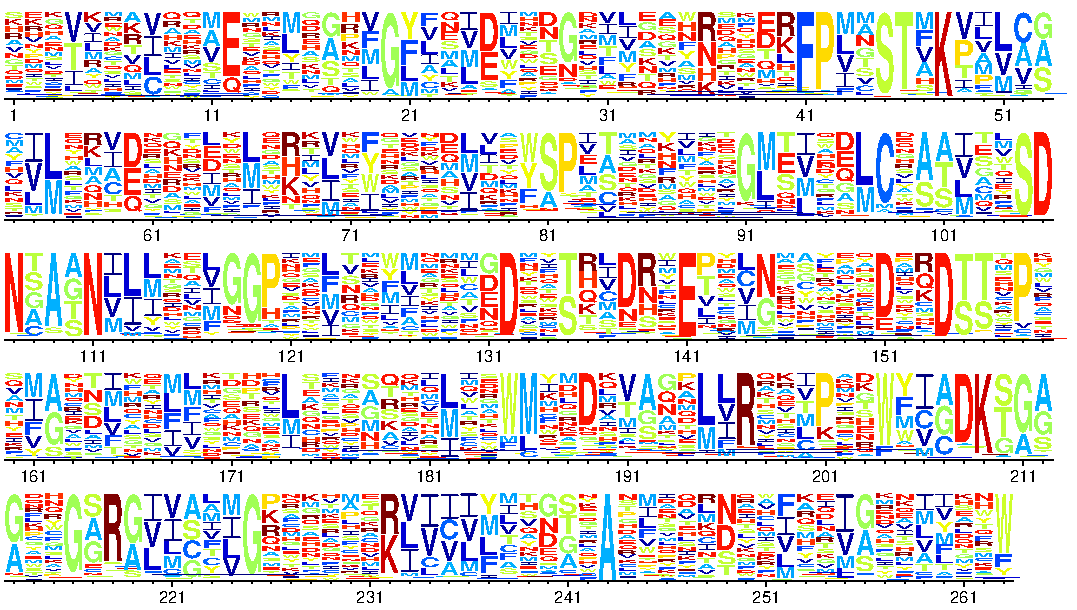
\includegraphics[width=\textwidth, page=1] {prefs_plots_lactamase_stiffler.pdf}
    \caption[Deep mutational scanning profile]{
    Site-specific deep mutational scanning data on beta-lactamase of~\citep{Stiffler2015}.
    The analysis is performed using phydms~\citep{Hilton2017}.}
    \label{fig:intro-deep-mut-profile}
\end{figure}
Even though it is possible to compare estimated fitness profiles under phylogenetic codon models with predicted profiles under biophysical modeling, I argue that this congruence and confrontation is scarcely made.

\subsection{Structurally-constrained site-interdependent codon models}

It has long been realized that inter-residue interactions within the protein conformation lead to amino acid fixation probabilities that are dependent upon the amino-acid present at other sites.
More generally, site-specific fixation probabilities may change along an evolutionary trajectory because the selection coefficient of a given mutation may depend on the specific sequence background in which it occurs~\citep{Goldstein2016}.
However, either classical codon models or mechanistic codon models rely on the assumption of site-independence, where each site of the protein is modeled as an independent Markov process.
Accordingly, each site is considered separately, and defines an independent Markov substitution process along the branches of a tree.

From a modeling and inference perspective, accounting for epistasis is challenging both in terms of parametrization and computational complexity~\citep{Manhart2014}.
Means of relaxing this assumption have been pursued, usually with dependence introduced between a limited number of sites~\citep{Felsenstein1996}.
In particular, models explicitly treating protein structure and site inter-dependencies have been developed, recruiting a coarse-grained protein structure conjointly to a statistical potential scoring the compatibility between sequence and structure, in order to evaluate the probability of fixation of a given mutation~\citep{Robinson2003, Rodrigue2005}.

Subsequently, methods to assess the statistical fit of such computationally complex models had been developed~\citep{Rodrigue2009}, as well as refinement of statistical potentials~\citep{Kleinman2010}.
These structurally constrained models have been shown to fit data better than the corresponding models that ignore protein structure.
However, some of the available site-independent phylogenetic codon models still better fit to the data than structurally constrained models, possibly indicating that alternatives models should be explored in order to better incorporate structural constrain and protein biophysics.

Alternatively, assumption of site-independence can be understood as considering that substitution process at the level of site are averaged over time, where the dependencies to other sites are integrated over the course of the process.
As a result, statistical method relying on site-independent processes while accounting for other sites consist in obtaining the marginal process for a specific site, derived analytically from the joint process integrated over the other sites.
Projecting a joint process of several sites into a single site process leverages mean-field theory developed in statistical physics, and as been used to developed phylogenetic models accounting for protein structure~\citep{Chi2018} and protein stability~\citep{Arenas2015a, Arenas2017}.
Unfortunately, these methods are not parameterized directly in terms of parameters of evolution, namely mutation and effective population size, and the estimated fitness parameters can not be related to empirically determined parameters.

\section{General conclusions}

Finally, models of protein biophysics are appealing to evolutionary biologists since they are based on theoretical ground and can also be confronted to empirical data.
However, integration of protein biophysics models into the framework of phylogenetic inference is difficult, and inference models have to balance the trade-off between complexity and simplicity.
Moreover, I argue that phylogenetic model should be mechanistic in principle, or in other words they should be defined in terms of parameters that can be accessed by independent experimental means, such as to confront estimates.
As an example, analytical models of protein biophysics relating probability of fixation to molecular and thermodynamics parameters can be fitted to protein coding DNA sequences, and estimates can compared to their empirically determined counterpart, such as to verify and solidify the soundness of both phylogenetic inference and protein biophysics.